%Hauptdokument

\documentclass[11pt]{article}


%Vorspann

\usepackage[T1]{fontenc}
\usepackage[utf8x]{inputenc}

%\usepackage{ngerman}
\usepackage{graphicx}
\usepackage{anysize}
\usepackage{enumitem}
\usepackage{makeidx}
\usepackage{subfig}


\usepackage{blindtext,wrapfig}
\usepackage[headsepline]{scrpage2}
\pagestyle{scrheadings}


\setcounter{secnumdepth}{3}
\setcounter{tocdepth}{3}

\usepackage{hyperref}

\usepackage{color}
\definecolor{darkred}{rgb}{0.5,0.0,0.0}
\hypersetup{colorlinks, linkcolor=darkred}

\renewcommand{\figurename}{Abbildung}


\usepackage{makeidx}
\makeindex


\begin{document}

\begin{titlepage}

\author{Lars Strölin, Michael Geigges, Ilja Kononenko} 
\title{Grafikrechner Entwicklerdokumentation} 
\date{10. Juli 2018} 
\maketitle

\setcounter{page}{1}

%Titelbild
\begin{figure}[ht]
	\centering
	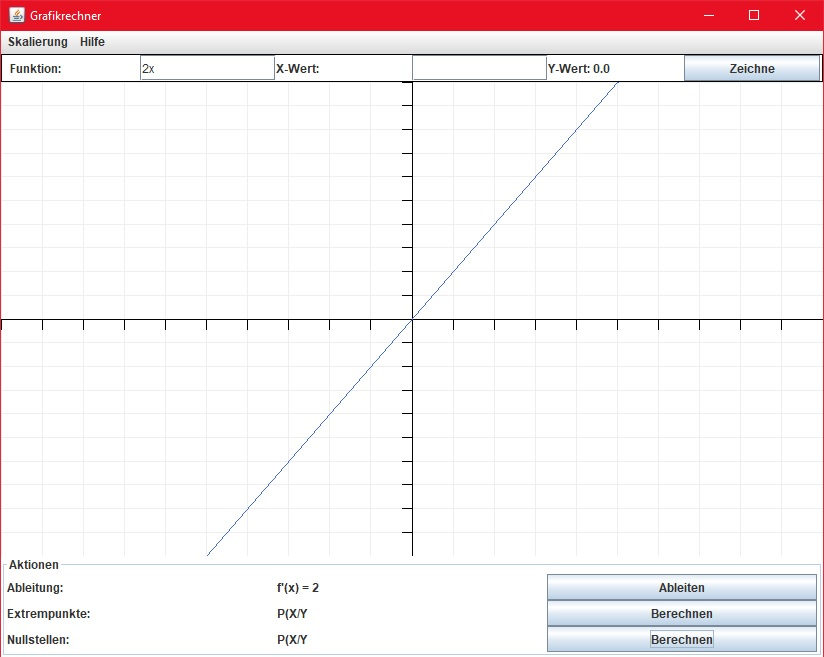
\includegraphics[width=1.0\textwidth]{Bilder/GR_1.jpg}
	\caption{Grafikrechner}
\end{figure}

\end{titlepage}


\tableofcontents
\newpage


%Ausgelagerte Elemente
%Vorwort

\ihead{\headmark}
\ohead{Lars Strölin, Michael Geigges, Ilja Kononenko}
\automark{section}
\cfoot{\pagemark}


\section{Vorwort}
Diese Entwicklerdokumentation dient allein nur für die reibungslose Weiterentwicklung bzw. zeigt den aktuellen Aufbau des Grafikrechner-Programms. 
\newline
Hier werden die jeweiligen Themen bzw. Arbeitsfunktionen anhand von Klassendiagrammen, Sequenzdiagrammen und falls notwendig Struktogrammen erklärt und wichtige Funktionen dargestellt, sowie Ansatzpunkte zur Weiterentwicklung weiter gegeben. Damit der nachfolgende Entwickler die Arbeit von uns  schnell nachvollziehen und in diese leicht einsteigen kann, wird die Erklärung so kurz wie möglich gehalten und nur das Wichtigste erklärt. Daher sind alle leicht nachvollziehbaren Sachen vom Quellcode bzw. vom Javadoc zu entnehmen. 
Am Ende dieser Entwicklerdokumentation werden die größten Schwierigkeiten und Probleme aufsummiert und geschildert, damit der nachfolgende Entwickler davon eine grobe Einschätzung bekommen kann, was für Problematiken auf ihn in diesem Projekt zu kommen werden.




\newpage
%Aufbau

\ihead{\headmark}
\ohead{Lars Strölin, Michael Geigges, Ilja Kononenko}
\automark{section}
\cfoot{\pagemark}


\section{Aufbau}
%%Funktion

\ihead{\headmark}
\ohead{Lars Strölin, Michael Geigges, Ilja Kononenko}
\automark{section}
\cfoot{\pagemark}


\section{Funktion}

\textbf{Funktionen und Aufbau im Überblick:}

\begin{enumerate}[label=\Roman*)]
	\item Eingabe
	\item Zeichnen
	\item Berechnen
	\item Hilfe
\end{enumerate}

%-----------------------------------------------------------------------------------------

\subsection{Eingabe}
Um eine Funktion eingeben zu können verwendet man das erste Eingabefeld links oben neben der Beschriftung "Funktion: ". Dort kann man dann eine X-beliebige Funktion eingeben, welche später auf dem KOS angezeigt werden kann.
\newline
Für die Berechnung eines Y-Wertes gibt es das zweite Eingabefeld rechts daneben mit der Beschriftung "X-Wert: ". Hier kann auch einen komplett beliebigen Wert mit einem "X" eingeben.

\begin{figure}[ht]
	\centering
	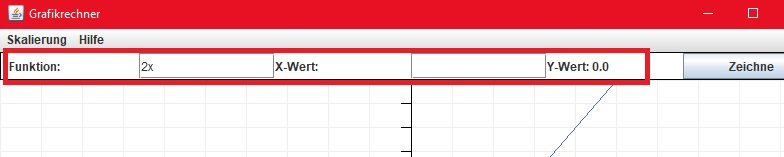
\includegraphics[width=1.0\textwidth]{Bilder/GR_2.jpg}
	\caption{Erstes und zweites Eingabefeld}
\end{figure}

%-----------------------------------------------------------------------------------------

\subsection{Zeichnen}
Um die Funktion dann auf dem Koordinatensystem anzeigen zu lassen benutzt man rechts oben im Eck den "Zeichne"-Button. Danach wird in anderer Farbe sofort auf dem Feld die Funktion gezeichnet und und korrekt angezeigt.

\begin{figure}[ht]
	\centering
	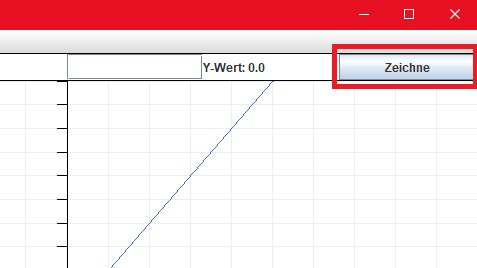
\includegraphics[width=0.6\textwidth]{Bilder/GR_3.jpg}
	\caption{Zeichne-Button}
\end{figure}


\subsubsection{Skalierung}
Die standardmäßige Größe des KOS (Koordinatensystem) beträgt in alle vier Richtungen 10 bzw. -10.
Aufgrund dessen, dass gewisse Funktionen ihre wichtigen Punkte in darüber liegenden Werten besitzen, oder der Benutzer einfach einen anderen Bereich gerne anschauen will, gibt es eine Einstellung für die Skalierung. 
\newline
In der Menüleiste gibt es links oben als erster Punkt das Menüitem Skalierung. Drückt man auf diesen Punkt öffnet sich ein Unterpunkt und unter dort kann man dann über ein Fenster, welches sich dann extra öffnet, die vier Werte der Skalierung manuell seinen Wünschen anpassen. Über den Punkt "Skalierung einstellen" werden die Werte auf der Anzeige übernommen. Der Punkt "Standard Skalierung" stellt die üblichen Werte 10 bzw. -10 wieder her.

\begin{figure}[ht]
	\begin{center}
		\subfloat[Menüitem Skalierung]{
		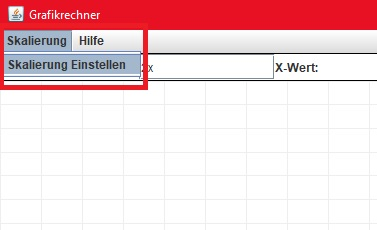
\includegraphics[width=0.4\textwidth]{Bilder/GR_4.jpg} }
	\hspace{1cm}
		\subfloat[Einstellungen für die Skalierung]{
		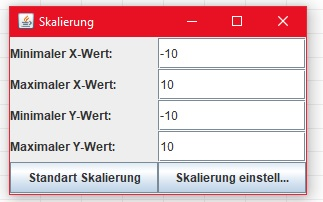
\includegraphics[width=0.4\textwidth]{Bilder/GR_5.jpg} }
	\end{center}
\end{figure}

%-----------------------------------------------------------------------------------------

\subsection{Berechnen}
Nach Eingabe einer Funktion im zweiten Eingabefeld gibt es rechts oben speziell für den Y-Wert ein Ausgabefeld. Um den Y-Wert zu erhalten muss man lediglich nach der Eingabe die "ENTER"-Taste drücken.

\subsubsection{Besondere Werte} 
In der Mathematik gibt es bestimmte Werte die von besonderer Bedeutung sind, wie z.B die Nullstellen, Hoch- und Tiefpunkte (Extrempunkte) oder die Ableitung. Auch dafür bietet das Programm unter dem KOS eine Lösung. Hier befinden sich jeweils drei Ausgabefelder mit einem "Berechne"-Button. Wird dieser nach einer korrekten Eingabe im ersten Eingabefeld gedrückt, werden die jeweiligen Werte berechnet und ausgegeben.

\begin{figure}[ht]
	\centering
	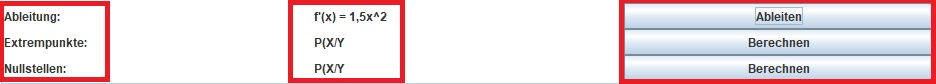
\includegraphics[width=1.0\textwidth]{Bilder/GR_6.jpg}
	\caption{Ausgabefelder für besondere Werte}
\end{figure}

\newpage

%-----------------------------------------------------------------------------------------

\subsection{Hilfe}
In der Menüleiste gibt es neben der Skalierung noch den zweiten Punkt "Hilfe". Dort kommt man zu den Unterpunkten "Anleitung" und "Über". 
\newline
Bei der Anleitung öffnet sich auch ein extra Fenster mit einer kleinen Anleitung um die Hauptfunktionen noch einmal zu erklären. 
\newline
Unter dem Punkt "Über" wird einem auch in ein einem extra Fenster die aktuelle Version des Programms und weitere Informationen angezeigt.

\begin{figure}[ht]
	\begin{center}
		\subfloat[Menüitem Hilfe]{
		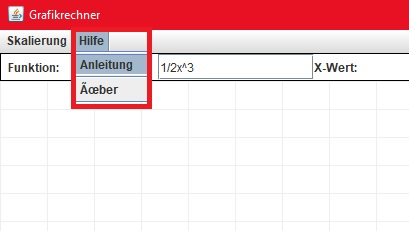
\includegraphics[width=0.4\textwidth]{Bilder/GR_7.jpg} }
	\hspace{1cm}
		\subfloat[Extrafenster für die Anleitung]{
		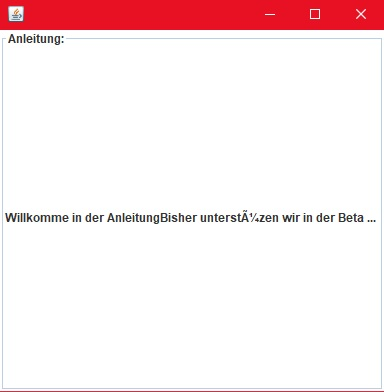
\includegraphics[width=0.4\textwidth]{Bilder/GR_8.jpg} }
	\end{center}
\end{figure}


%-----------------------------------------------------------------------------------------






%Vorwort

\ihead{\headmark}
\ohead{Lars Strölin, Michael Geigges, Ilja Kononenko}
\automark{section}
\cfoot{\pagemark}


\section{Fazit}

Im Großen und Ganzen ist es uns gelungen ein Programm zu entwickeln, welches durch Eingabe einer Funktion diese in einem Schaubild korrekt darstellt und dazu auch besondere Werte, wie z.B. Nullstellen und Extrempunkte ausrechnet. Es war aber dennoch für uns sehr schwierig diese Aufgabe zu realisieren, da wir uns erst Gedanken machen mussten, wie wir die Erstellung unseres Programms angehen und vor allem wie wir die mathematischen Formeln programmieren.\\

Die größten Schwierigkeiten und Problematiken waren deshalb die Codes für die Ausrechnung der besonderen Werte für unser Programm zu entwickeln. 
Doch genau aus diesem Grund sind wir zufrieden es geschafft zu haben und können jetzt im Programm Verbesserungen durchführen. Die Oberfläche muss auf jeden Fall noch benutzerfreundlicher gestaltet und zum Teil automatisiert werden.\\

Außerdem hatten wir uns eigentlich vorgenommen eine Funktion zu entwickeln, in der man bestimmte Funktionen abspeichern und wieder aufrufen kann, da uns aber die Zeit dazu gefehlt hat und diese Funktionen optional waren, fielen sie für die Abgabe des jetzigen Programms raus.


\addcontentsline{toc}{section}{Stichwortverzeichnis}
\printindex

\end{document}